%& /Users/ziky/.cache/org-persist/b5/4009bf-1c6d-4252-aa94-84b94b3f4885-3006af205b6e876d903c956a87857e13
% Created 2026-01-31 Sat 17:05
% Intended LaTeX compiler: pdflatex
\documentclass[11pt]{article}
\usepackage[utf8]{inputenc}
\usepackage[T1]{fontenc}
\usepackage{amsmath}
\usepackage{amssymb}
\usepackage{capt-of}
\usepackage{hyperref}
\setlength{\abovedisplayskip}{0pt}
\setlength{\belowdisplayskip}{0pt}
\usepackage[a4paper, margin=1in]{geometry}

%% ox-latex features:
%   !announce-start, !guess-pollyglossia, !guess-babel, !guess-inputenc,
%   maths, image, !announce-end.

\usepackage{amsmath}
\usepackage{amssymb}

\usepackage{graphicx}

%% end ox-latex features


% end precompiled preamble
\ifcsname endofdump\endcsname\endofdump\fi

\author{Ziky Zhang}
\date{\today}
\title{Jan 27th Class Notes}
\hypersetup{
 pdfauthor={Ziky Zhang},
 pdftitle={Jan 27th Class Notes},
 pdfkeywords={},
 pdfsubject={},
 pdfcreator={},
 pdflang={English}}
\begin{document}

\maketitle
Photoelectric Effect and H atom emission \& absorption phenomeno successfully model of energy transitions associated with light.

\begin{center}
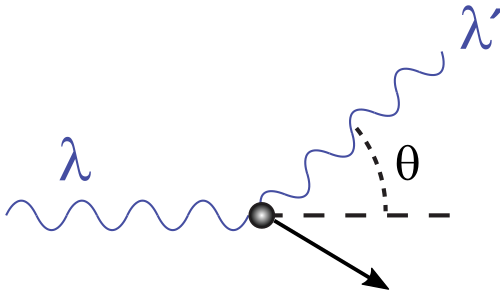
\includegraphics[height=4cm]{./img/Compton-scattering.svg.png}
\label{orga321911}
\end{center}

Wave model predicts \(\lambda' = \lambda\) regardless of \(\theta\);
\begin{itemize}
\item the amplitude of outgooing wave is smaller than incoming wave.
\end{itemize}
The Wave model fails.

Arthur Compton used \(E_{\gamma} =hf\) \& \(p_{\gamma} \frac{E_{\gamma}}{c}\) for photon incoming and outgoing
\(\lambda' - \lambda = \frac{h}{m_e c} (1 - \cos\theta)\)
Particle model predicts what is seen in experiment and matches experiment.
Divide both sides by \(c\).
\begin{align*}
\frac{1}{c}(\lambda' - \lambda) &= \frac{h}{m_ec} (1 - \cos \theta) \\
\text{take the equation from the wave model: }\frac{1}{f} = \frac{\lambda}{c} \\
\frac{1}{f'} - \frac{1}{f} &= \frac{h}{m_e c}(1 - \cos \theta)
\end{align*}
\(\frac{h}{m_e c} = 0.002426 \mathrm{nm}\) is what refers to as Compton wavelength.
\(\frac{hc}{m_e c^2} = \frac{1240 \mathrm{eV \cdot nm}}{.511 \mathrm{MeV}}\)

Light still does behave like a wave
But particles are acting like waves as well.
\begin{itemize}
\item Bounce off of crystals
\item Travel through small openings
\end{itemize}
Louis de Broglie assigned wavelength of particles in his PhD thesis, later on become a Nobel prize winning piece of thesis \(\lambda = \frac{h}{P}\), where \(P\) is the quantitatively leads to the correct differaction and interference patterns.
\end{document}
